\addcontentsline{toc}{section}{Вариант 3}
\section*{Вариант 3}

\subsubsection*{1}

\textit{Задание.} Что вероятней: выиграть у равносильного противника 3 шахматных партии из 4 или 5 партий из 8?

\textit{Решение.} Найдём вероятность выиграть 3 шахматные партии из четырёх.
Пространство элементарных событий состоит из $ \left| \Omega_1 \right| = 2^4$ элементов,
так как каждую из четырёх партий можно выиграть или проиграть.
Введём событие $A =$ \{3 партии из четырёх будут удачными\}.
Нужно выбрать одну партию из четырёх, которая не будет удачной --- это $C_4^1 = \left| A \right| $.
Тогда вероятность этого события равна
$$P \left( A \right) =
\frac{ \left| A \right| }{ \left| \Omega_1 \right| } =
\frac{C_4^1}{2^4} =
\frac{4}{4^2} =
\frac{1}{4}.$$

Найдём вероятность выиграть 4 шахматные партии из восьми.
Пространство элементарных событий в данном случае состоит из $ \left| \Omega_2 \right| = 2^8$ элементов.
Пусть событие $B =$ \{5 партий из восьми закончатся победой\}.
Нужно выбрать 5 партий из восьми, которые закончатся победой --- это
$$ \left| B \right| =
C_8^5 =
\frac{8!}{5! \cdot 3!} =
\frac{6 \cdot 7 \cdot 8}{2 \cdot 3} =
7 \cdot 8.$$
Тогда вероятность этого события равна
$$P \left( B \right) =
\frac{ \left| B \right| }{ \left| \Omega \right| } =
\frac{7  \cdot 8}{2^8} =
\frac{7}{2^5} =
\frac{7}{32}.$$

Сравним две полученные вероятности.
Для этого первую умножим на 8:
$$ \frac{8}{8} \cdot \frac{1}{4} =
\frac{8}{32}.$$
Видим, что
$$ \frac{8}{32} > \frac{7}{32},$$
поэтому $P \left( A \right) > P \left( B \right) $.
Тогда вероятность выиграть 3 шахматные партии из четырёх больше, чем вероятность выиграть 5 партий из восьми.

\subsubsection*{2}

\textit{Задание.} В сундуке лежат 9 красных, 6 синих и 5 зелёных пуговиц.
Наугад вынули 2 пуговицы.
Найдите вероятность того, что пуговицы разного цвета, если известно, что среди них нет зелёных.

\textit{Решение.} Опишем событие $A =$ \{среди двух пуговиц нет зелёных\}.
Возможны варианты: (красная, красная), (синяя, синяя), (красная, синяя), (синяя, красная).
Вероятность того, что вытянем одну красную и одну синюю пуговицу, равна
$$ \frac{9}{20} \cdot \frac{6}{19}.$$
Вероятность того, что две пуговицы будут красными, равна
$$ \frac{9}{20} \cdot \frac{8}{19}.$$
Наконец, вероятность того, что две пуговицы будут синими, равна
$$ \frac{6}{20} \cdot \frac{5}{19}.$$
Тогда по правилу суммы имеем вероятность указанного события:
\begin{equation*}
\begin{split}
P \left( A \right) =
\frac{2 \cdot 9 \cdot 6}{20 \cdot 19} + \frac{9 \cdot 8}{20 \cdot 19} + \frac{6 \cdot 5}{20 \cdot 19} =
\frac{9 \cdot 6 + 9 \cdot 4 + 3 \cdot 5}{10 \cdot 19} =
\frac{54 + 36 + 15}{10 \cdot 19} = \\
= \frac{105}{10 \cdot 19} =
\frac{21}{2 \cdot 19}.
\end{split}
\end{equation*}

Введём событие $B =$ \{пуговицы оказались разного цвета\}.
Найдём пересечение двух событий: $A \cap B =$ \{пуговицы оказались разного цвета, и среди них нет зелёных\}.
Есть два варианта: (красный, синий), (синий, красный).
Вероятность этого пересечения равна
$$P \left( A \cap B \right) =
\frac{2 \cdot 9 \cdot 6}{20 \cdot 19} =
\frac{9 \cdot 6}{10 \cdot 19} =
\frac{9 \cdot 3}{5 \cdot 19}.$$

Тогда по формуле для условной вероятность получаем, что
$$P \left( \left. B \right| A \right) =
\frac{P \left( A \cap B \right) }{P \left( A \right) } =
\frac{9 \cdot 3}{5 \cdot 19} \cdot \frac{2 \cdot 19}{21} =
\frac{9 \cdot 2}{5 \cdot 7} =
\frac{18}{35}.$$

\subsubsection*{3}

\textit{Задание.} На отрезок наугад брошены две точки.
Найдите вероятность того, что левый из трёх образованных отрезков будет самым коротким.

\textit{Решение.} Пусть отрезок начинается в точке 0 и заканчивается в точке $c$.
Выбираем на нём наугад две точки: точку $a$ и точку $b$, причём $a$ лежит не правее $b$ (рис. \ref{fig:24}).

Тогда пространство элементарных исходов имеет вид $ \Omega =  \\
= \left\{ \left( a, b \right): 0 \leq a \leq b \leq c \right\} $.
Изобразив его на плоскости, видим, что это прямоугольный треугольник с катетами длиной $c$ (рис. \ref{fig:33}).

\begin{figure}[h!]
  \centering
  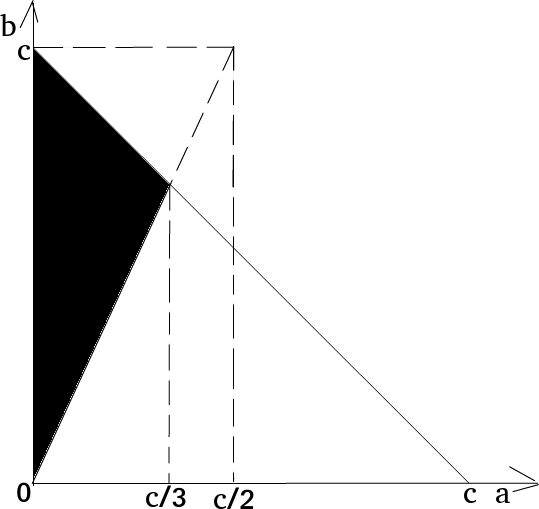
\includegraphics[width=.4\textwidth]{./pictures/t1v3_3.png}
  \caption{Пространство элементарных событий $ \Omega$ и событие $A$}
  \label{fig:33}
\end{figure}

Площадь треугольника равна
$$S_{ \Omega } =
\frac{1}{2} \cdot c \cdot c =
\frac{c^2}{2}.$$

Пусть событие $A = \left\{ \left( a, b \right) \in \Omega: a \leq b-a, a \leq c-b \right\} $.
Изобразив его на рисунке, видим, что это треугольник, образованный прямой $b = c - a$, прямой $b = 2a$ и одним из катетов исходного треугольника.
Его площадь найдём с помощью интеграла:
$$S_1 =
\int \limits_0^{ \frac{c}{3} } \left( c - a \right) da =
\left. \left( ca - \frac{a^2}{2} \right) \right|_0^{ \frac{c}{3} } =
c \cdot \frac{c}{3} - \frac{c^2}{9 \cdot 2} =
\frac{c^2}{3} - \frac{c^2}{18} =
\frac{6c^2 - c^2}{18} =
\frac{5c^2}{18}.$$
От этой площади нужно отнять площадь треугольника под прямой $b = 2a$.
Она равна
$$S_2 =
\frac{1}{2} \cdot \frac{c}{3} \cdot \frac{2c}{3} =
\frac{c^2}{9}.$$

Площадь треугольника равна
$$S_A =
S_1 - S_2 =
\frac{c^2}{6}.$$

Тогда вероятность этого события равна
$$P \left( A \right) =
\frac{S_A}{S_{ \Omega }} =
\frac{1}{3}.$$

\subsubsection*{4}

\textit{Задание.} Частица совершает случайное симметрическое блуждание на прямой, делая шаг вправо или влево с вероятностью $1/2$.
Найдите вероятность того, что через $2n$ шагов частица впервые вернётся в исходную точку.

\textit{Решение.} Задача изображена на рисунке \ref{fig:34}.

\begin{figure}[h!]
  \centering
  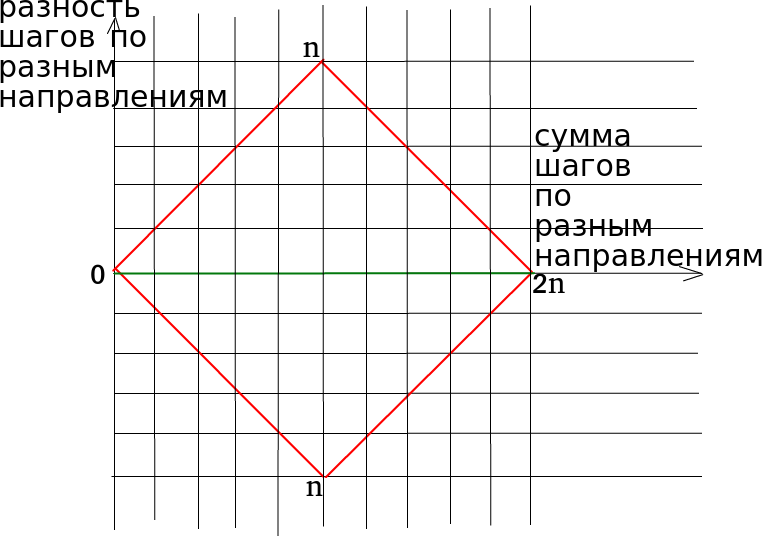
\includegraphics[width=.4\textwidth]{./pictures/t1v3_4.png}
  \caption{Задача про случайное блуждание частицы на прямой}
  \label{fig:34}
\end{figure}

Красным обозначены крайние пути, зелёным --- линия, которую нельзя пересекать.
Перевернём изображение (рис. \ref{fig:341}).

\begin{figure}[h!]
  \centering
  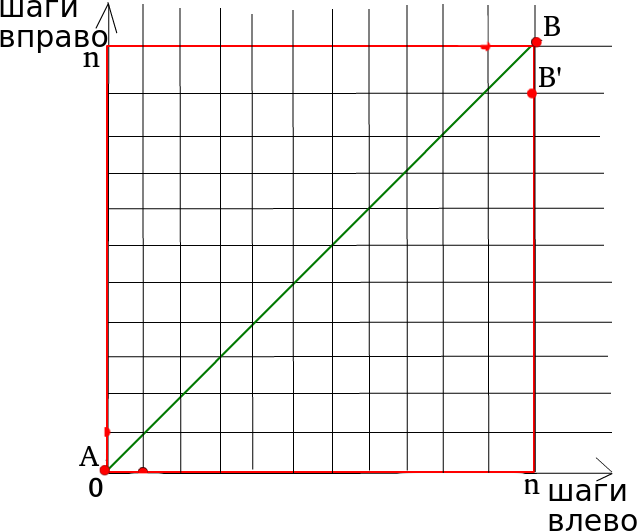
\includegraphics[width=.4\textwidth]{./pictures/t1v3_41.png}
  \caption{Метод отражений}
  \label{fig:341}
\end{figure}

Всего путей
$$ \left| \Omega \right| =
2^{2n}.$$

Начальная точка --- точка $A$, конечная --- точка $B$.
Всего путей из $A$ в $B$ существует
$$ \left| A \rightarrow B \right| =
C_{n+n}^n =
C_{2n}^n =
\frac{ \left( 2n \right)!}{n!n!}.$$

Путей, которые пересекают диагональ будет
$$ \left| A \rightarrow B' \right| =
C_{n+n-1}^n =
C_{2n-1}^n =
\frac{ \left( 2n-1 \right)!}{n! \left( n-1 \right)!}.$$

Тогда путей, которые не пересекают диагональ будет
\begin{equation*}
\begin{split}
2 \left( \left| A \rightarrow B \right| - \left| A \rightarrow B' \right| \right) =
2 \cdot \left( \frac{ \left( 2n \right)!}{n!n!} - \frac{ \left( 2n-1 \right)!}{n! \left( n-1 \right)!} \right) = \\
= 2 \left( \frac{ \left( 2n \right)!}{n! \left( n-1 \right)!n} - \frac{ \left( 2n-1 \right)!}{n! \left( n-1 \right)!} \right) =
2 \cdot \frac{ \left( 2n \right)! - \left( 2n-1 \right)!n}{n!n!} = \\
= 2 \cdot \frac{ \left( 2n-1 \right)! \left( 2n-n \right)}{n!n!} =
\frac{2 \left( 2n-1 \right)!n}{n!n!} =
\frac{2 \left( 2n-1 \right)!}{n! \left( n-1 \right)!},
\end{split}
\end{equation*}
так как частица может двигаться и вправо, и влево.

Тогда вероятность указанного в условии задачи события равна
$$P =
\frac{2 \left( 2n-1 \right)!}{n! \left( n-1 \right)! \cdot 2^{2n}} =
\frac{\left( 2n-1 \right)!}{n! \left( n-1 \right)! \cdot 2^{2n-1}}.$$

\subsubsection*{5}

\textit{Задание.}
Среди 5 стрелков есть 3 хороших, которые метко стреляют с вероятностью $0.8$, и 2 средних, которые попадают в цель с вероятностью $0.5$.
Вызвали наугад двух стрелков, они выстрелили по мишени и оба попали.
Найдите вероятность того, что стреляли два средних стрелка.

\textit{Решение.}
Введём событие $A =$ \{два стрелка попали по мишени\} и гипотезы о том,
каких стрелков вызвали: $H_1 =$ \{оба стрелка были хорошими\},
$H_2 =$ \{оба стрелка были средними\}, $H_3 =$ \{первый стрелок был хорошим, а второй --- средним\}, $H_4 =$ \{первый стрелок был средним, а второй хорошим\}.
Нужно найти вероятность
$$P \left( \left. H_2 \right| A \right) =
\frac{P \left( \left. A \right| H_2 \right) P \left( H_2 \right) }{ \sum \limits_{i=1}^4 P \left( \left. A \right| H_i \right) P \left( H_i \right) }.$$

Вероятность того, что выбрали два хороших стрелка равна
$$P \left( H_1 \right) =
\frac{3}{5} \cdot \frac{2}{4} =
\frac{3}{5} \cdot \frac{1}{2} =
\frac{3}{10}.$$

Вероятность того, что выбрали два средних стрелка равна
$$P \left( H_2 \right) =
\frac{2}{5} \cdot \frac{1}{4} =
\frac{1}{5 \cdot 2} =
\frac{1}{10}.$$

Вероятность того, что один из стрелков был хорошим, а второй --- средним равна
$$P \left( H_3 \right) =
P \left( H_4 \right) =
\frac{3}{5} \cdot \frac{2}{4} =
\frac{3}{10}.$$

Найдём условные вероятности:
\begin{equation*}
\begin{split}
P \left( \left. A \right| H_1 \right) =
\frac{8}{10} \cdot \frac{8}{10} =
\frac{4}{5} \cdot \frac{4}{5} =
\frac{16}{25}, \,
P \left( \left. A \right| H_2 \right) =
\frac{1}{2} \cdot \frac{1}{2} =
\frac{1}{4}, \,
P \left( \left. A \right| H_3 \right) = \\
= P \left( \left. A \right| H_4 \right) =
\frac{8}{10} \cdot \frac{1}{2} =
\frac{4}{5 \cdot 2} =
\frac{2}{5}.
\end{split}
\end{equation*}

Тогда по формуле Байеса получаем
$$P \left( \left. H_2 \right| A \right) =
\frac{ \frac{1}{4} \cdot \frac{1}{10} }{ \frac{3}{10} \cdot \frac{16}{25} + \frac{1}{4} \cdot \frac{1}{10} + 2 \cdot \frac{3}{10} \cdot \frac{2}{5} }$$
